\documentclass[margin=0mm, innermargin=3cm, blockverticalspace=15mm, colspace=15mm, subcolspace=8mm, a0paper, titleinnsersep = 0pt]{tikzposter}
\usepackage{graphicx} 
\usepackage[utf8]{inputenc}
\usepackage{xcolor}
\usepackage[ngerman]{babel}
\usepackage{tikz}
\tikzposterlatexaffectionproofoff %Tikzposter Wasserzeichen ausblenden
\usetikzlibrary{babel}
\setlength{\columnsep}{2cm}
\usepackage[backend=biber,style=alphabetic,]{biblatex}

\bibliography{Literatur}

%Abbildungsreferenzen Deutsch
\addto\captionsngerman{
  \renewcommand{\figurename}{Abb.}
  \renewcommand{\tablename}{Tab.}
}
\newcommand{\protfin}{prot-fin}
\newcommand{\bottomnode}[2]{
    \node[above right,
        outer sep=0pt,
        fill opacity=0,
        line width=0mm,
        text opacity=1,
        minimum width=80cm,
        minimum height=6cm,
        align=center,font=\Huge,
        draw=none,fill=white] at ([shift={(0.5*\pgflinewidth,0.5*\pgflinewidth)}]-40,#1){#2}
}

%Titel
\title{\parbox{0.75\linewidth}{\centering \protfin \\ Das SHAZAM für Proteinerkennung?}}

%Farbpalette in TH-Farbe von Originalvorlage
\definecolorpalette{thpalette} {
    \definecolor{thblue}{RGB}{0,91,153}
}

%Hintergrund: Rahmen etc.
\definebackgroundstyle{frame}{
    %Aussenrahmen
    \draw[inner sep=0pt, line width=30pt, color=thblue, fill=white]
    (-40,-57) rectangle (40, 57);
    %Linien box Praxisphase von x,y
    \draw[line width=15pt, color=thblue] (-40,45) -- (40,45);
    \draw[line width=15pt, color=thblue] (-40,38) -- (40,38);
    %Linien box Durchgefuehrt bei: Betrieb, Ort
    % \draw[line width=15pt, color=thblue] (-40,-45) -- (40,-45);
    \draw[line width=15pt, color=thblue] (-40,-51) -- (40,-51);
}

%Titel Style
\definetitlestyle{thtitle}{
    width=\paperwidth, roundedcorners=0, linewidth=0pt, innersep=1.5cm,
    titletotopverticalspace=5cm, titletoblockverticalspace=7cm,
    titlegraphictotitledistance=1pt, titletextscale=1
}{}

%Block Style
\defineblockstyle{thblocks}{
    titlewidthscale=0.9,
    bodywidthscale=1,
    titleleft,
    titleoffsetx=0pt,
    titleoffsety=3mm,
    bodyoffsetx=0mm,
    bodyoffsety=19mm,
    bodyverticalshift=18mm,
    roundedcorners=5,
    linewidth=2pt,
    titleinnersep=6mm,
    bodyinnersep=1cm
}{
\draw[color=thblue, fill=blockbodybgcolor] (blockbody.south west)
rectangle (blockbody.north east);
\ifBlockHasTitle
\draw[color=thblue, fill=thblue] (blocktitle.south west)
rectangle (blocktitle.north east);
\fi
}
\defineblockstyle{picture}{
    titlewidthscale=0.9,
    bodywidthscale=1,
    titleleft,
    titleoffsetx=0pt,
    titleoffsety=0mm,
    bodyoffsetx=0mm,
    bodyoffsety=0mm,
    bodyverticalshift=3mm,
    roundedcorners=0,
    linewidth=2pt,
    titleinnersep=0mm,
    bodyinnersep=0cm
}{
% \draw[color=thblue, fill=blockbodybgcolor] (blockbody.south west)
% rectangle (blockbody.north east);
% \ifBlockHasTitle
% \draw[color=thblue, fill=thblue] (blocktitle.south west)
% rectangle (blocktitle.north east);
% \fi
}

%TH layout definieren
\definelayouttheme{th}{
    \usebackgroundstyle{frame}
    \usecolorpalette{thpalette}
    \usetitlestyle{thtitle}
    \useblockstyle{thblocks}
}

\usetheme{th} 

\begin{document}
%Logos einfuegen
% \node (betrieb) at (32, 51) {
\includegraphics[width=10cm]{unilogo.png}};
\node (thlogo) at (-28.5, 50.5) {
\includegraphics[width=10cm]{unilogo.png}};

%Praxisphase von Vorname Name
\bottomnode{38.4}{Praxisphase von Franz-Eric Sill\\Durchgeführt bei: Prof. Asis Hallab, TH Bingen};

%Durchgefuehrt bei Firma, Ort
% \bottomnode{-51}{Durchgeführt bei: Prof. Asis Hallab, TH Bingen};

%Studiengang Angewandte Bioinformatik
\bottomnode{-57}{Studiengang Angewandte Bioinformatik};
asd
\maketitle[]
\begin{columns}
\column{}

%Bloecke mit Inhalt
% \block[bodyverticalshift=0mm]{}{
\block{Einleitung}{
    Als SHAZAM ist eine Anwendung bekannt, die Musiktitel in Sekundenschnelle anhand von ebenso kurzen Tonaufnahmen erkennt. Der Kern des Algorithmus gleicht hierbei die Struktur der Aufnahme mit einer Datenbank ab, die mit Millionen von Songs gefüttert wurde und liefert den besten Treffer als Ergebnis \cite{wang}.

    Doch wäre das auch für Proteine möglich?

    Aktuell sind Alignments von den Aminosäureketten eine sehr populäre und effiziente Methode, um Proteine und deren funktionsgleiche Verwandte über Sequenzähnlichkeit zu erkennen. Bekannte Tools hierfür sind bspw. BLAST und DIAMOND.\
    Das Problem hierbei ist, dass mit zunehmender evolutionärer Distanz zwischen Sequenzen gefundene Homologien nicht mehr signifikant von zufälliger Ähnlichkeit zu unterscheiden sind. Es gilt das Basiskonzept von Struktur und Funktion, dennoch wird hier keine Ähnlichkeit auf Basis der Struktur festgestellt, da die letztendliche Tertiärstruktur schwer vorhersehbar ist und lediglich die aufgetretenen Aminosäuren verglichen werden.
    Wenn diese Vorgehensweise also nicht immer ideal ist und SHAZAM Musik auf Basis struktureller Information erkennt, wäre es doch vielleicht möglich, dass der zugrundeliegende Algorithmus in den physikalischen Eigenschaften der Proteinsequenzen strukturelle Information findet, die spezifisch für das Protein und vielleicht auch seine Verwandten ist.
}
\end{columns}
\begin{columns}
    
    % http://dx.doi.org/10.1007/BF01025492 - Kidera
    \column{0.66}
    \block{Methode}{
        % Erhalt numerischer Vektoren
        \textbf{Vorbereitung:} Voraussetzung für den Algorithmus ist ein numerischer Vektor, so wie es die digitale Tonspur bei SHAZAM darstellt. Um dies im proteinischen Kontext zu erreichen, wird in \protfin\ auf sogenannte Kidera-Faktoren zurückgegriffen. Diese Faktoren stammen aus einem Forschungsprojekt von Akinori Kidera, welches 1985 publiziert wurde \cite{kidera}. In diesem Projekt wurden für Aminosäuren 10 Faktoren ermittelt, mit denen die physikalischen Eigenschaften eines Proteins am meisten korrelieren, sodass nun eine Aminosäuresequenz pro Faktor in einen numerischen Vektor übersetzt werden, wobei ein höherer absoluter Wert für mehr Relevanz des jeweiligen Faktors steht.

        % Sammeln struktureller Information
        \vspace{2.25mm}
        \textbf{Sammeln von Strukturdaten:} Das Extrahieren von struktureller Information aus den erhaltenen Vektoren basiert auf der Short-Time-Fourier-Transformation (STFT), welche den Vektor intervallweise auf periodische Signale untersucht, wie z.B. dem wiederholten Auftreten von hydrophoben Aminosäuren im gleichen Abstand oder in der Musik ein Refrain oder dem Rhythmus. Die Frequenzen der auffälligsten Signale werden ausgewählt (Fig.~\ref{fig:1}), sodass über alle Intervalle eine sogenannte Constellation-Map entsteht, wobei das Reziproke einer Frequenz die Länge einer Periode in Aminosäuren angibt.

        % Hashing
        \vspace{2.25mm}
        \textbf{Hashing:} Die erhaltene Map wird nun elementweise gehashed, um einen effizienten Vergleich mit anderen Maps zu ermöglichen. Um das zu erzielen wird jede ausgewählte Frequenz mit jeder weiteren Frequenz der Folgeintervalle gepaart. Es werden also Kanten gebildet, wodurch die Map zu einem Graphen wird. Jede dieser Kanten bildet nun einen Hash, also einer Kombination aus den beiden Frequenzen/Kantenenden und der Kantenlänge. In einer Hashmap, also der Datenbank, wird sich folgend für den Hash die Position der Kante in der Constellation-Map gemerkt. Sollte ein Hash mehrfach vorkommen, so gilt dies nur für die letzte Position (Fig.~\ref{fig:1}).
    }
    \column{0.34}
    \useblockstyle{picture}
    \block{}{
        % \centering
        \begin{tikzfigure}[Frequenzselektion und Hashing]
            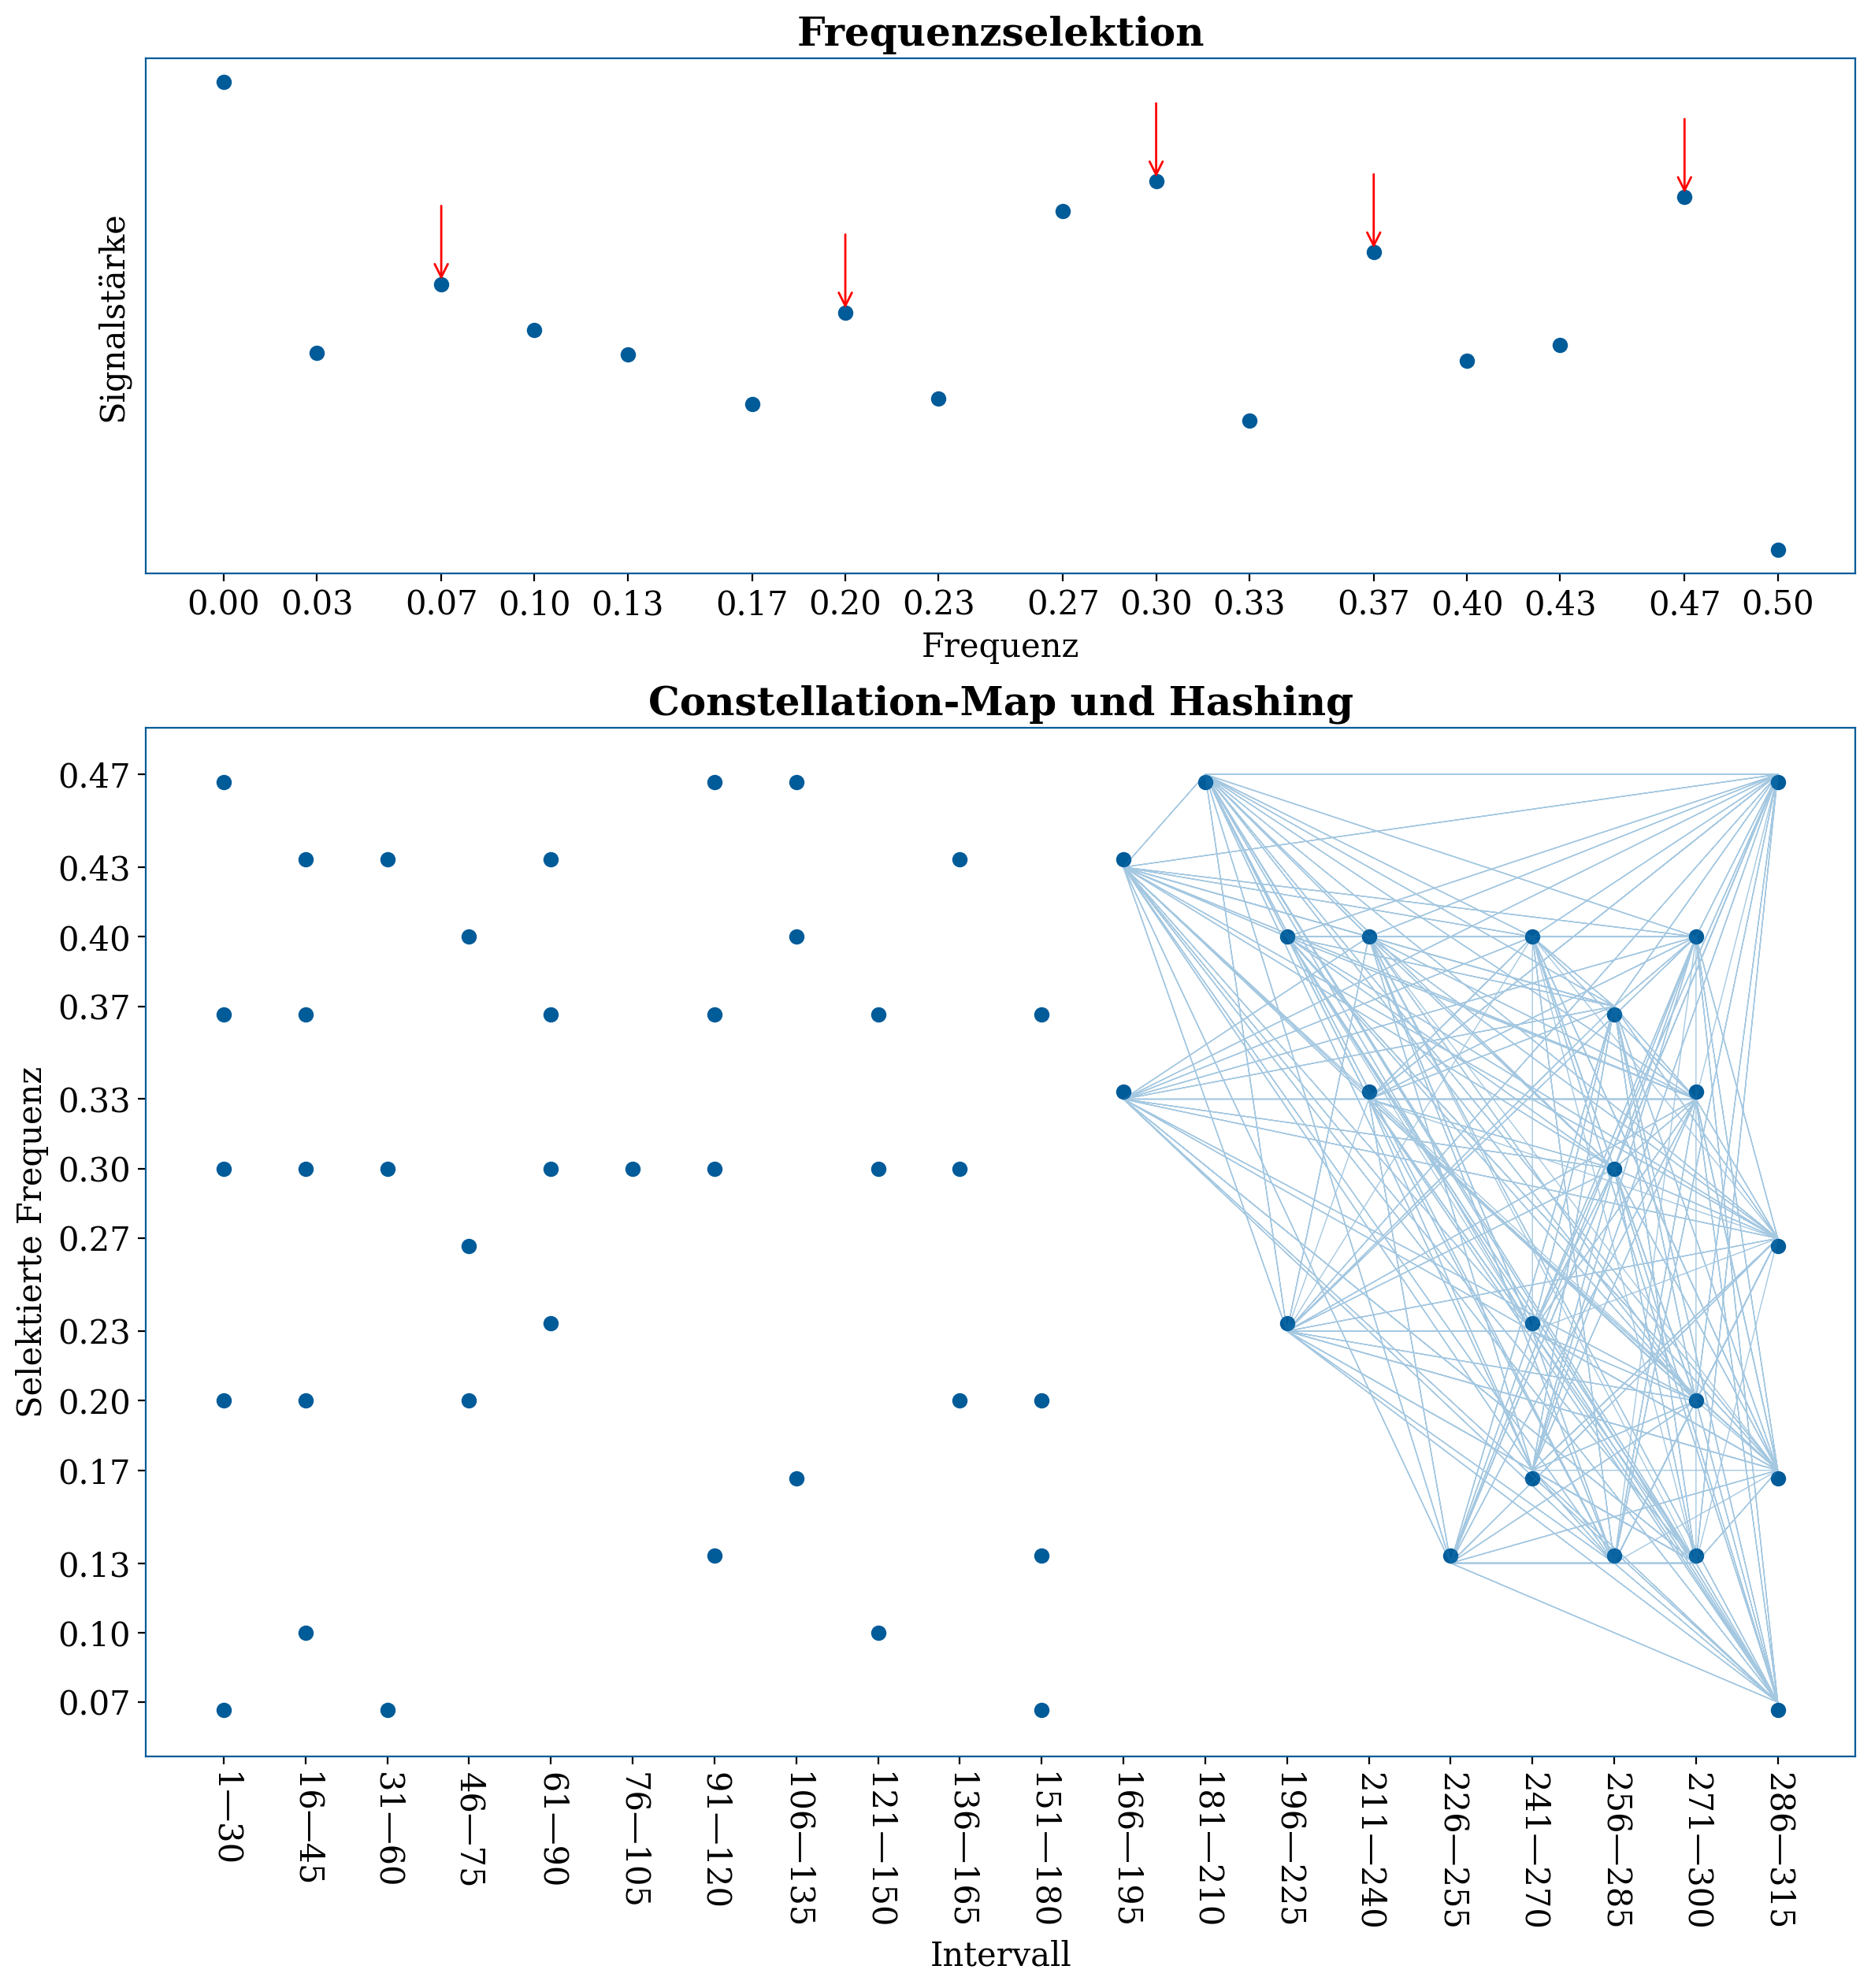
\includegraphics[scale=.77]{plot_method.png}
            \label{fig:1}
        \end{tikzfigure}
    }
\end{columns}
\begin{columns}
    \column{}
    \useblockstyle{thblocks}
    \block{Matching}{
        % Scoring/Map-Vergleich
        Nachdem eine Datenbank mit den Hashes verschiedener Trainings-Proteine (TP) trainiert wurde, wird sie verwendet, um Proteine zu erkennen. Dazu werden die Constellation-Map einer Eingabesequenz mit denen der TP verglichen. Jedes TP erhält einen Score (S1), der repräsentiert, wie viele seiner Hashes in Position mit der Eingabe übereinstimmen.

        Da sehr große Proteine potenziell kleine Proteine mit ihren Constellation-Maps als Subsequenz enthalten können, wird der Jaccard-Similarity-Index (JSI) aufmultipliziert, einem Maß, das die Übereinstimmung zweier Hash-Mengen A und B positionsunabhängig mit $\frac{|A \cap B|}{|A \cup B|}$ errechnet. Der Index nimmt somit  einen Wert von 0 an, wenn beide Mengen disjunkt sind, und nähert sich der 1 je größer die Schnittmenge ist, was somit die Schwäche des S1 ausbügelt.
    }
\end{columns}
\begin{columns}
    \column{.45}
    \useblockstyle{picture}
    \block{}{
        \begin{tikzfigure}[Erzielte Ergebnisse]
            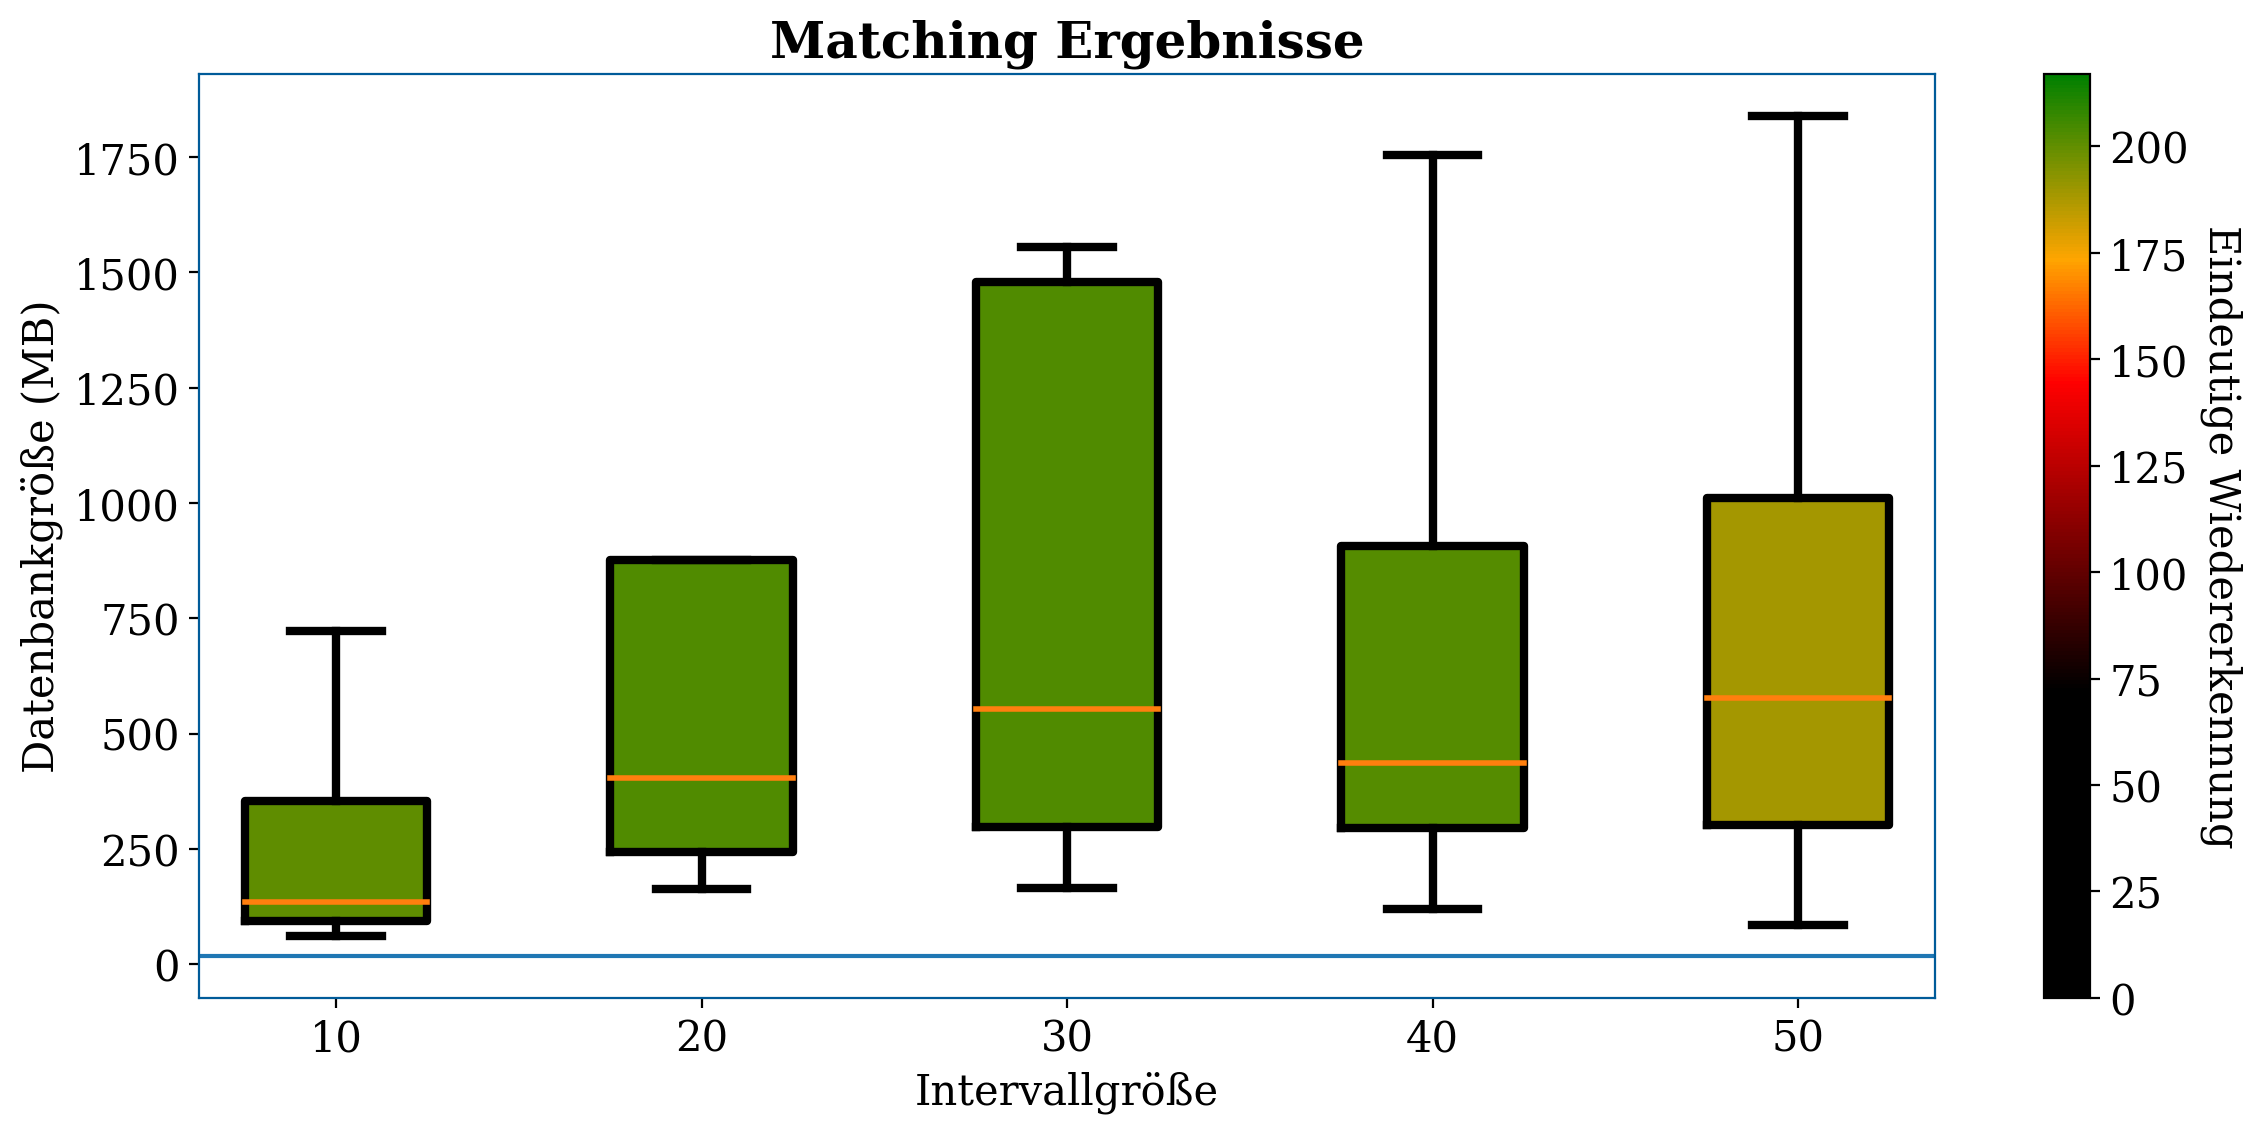
\includegraphics[scale=1.0285]{plot_previous.png}
            \label{fig:2}
        \end{tikzfigure}
    }
    \useblockstyle{thblocks}
    \block{Literatur}{\printbibliography[heading=none]}
    \column{.55}
    \useblockstyle{thblocks}
    \block{Performanz}{
        Um den Algorithmus von Musik auf Proteine abzustimmen, wurden bei der Erstellung der Constellation-Map verschiedene Parameter für die STFT durchprobiert, nämlich die Intervallgröße, der Abstand, wie weit das Intervall weitergeschoben wird, und die Anzahl an maximal selektierter Frequenzen. Als Trainingsdaten wurden circa 40.000 Pflanzenproteine verwendet und nachfolgend 217 vollständige Sequenzen möglichst funktionsverschiedener davon als Eingabe für das Matching, wobei lediglich die Hydrophobizität der Kidera Faktoren betrachtet wurde.

        In Fig.~\ref{fig:2} sind die Matching-Ergebnisse abgebildet, wobei die Boxen, gruppiert nach Intervallgröße, die Datenbankgrößen für die verschiedenen Parameterkonfigurationen wiedergeben, inklusive Median. Die Färbung einer Box stellt dar, wie viele der Eingabeproteine im  Mittel eindeutig erkannt wurden. Die Wiedererkennungsrate ist ziemlich hoch, aber die Datenbankgrößen ebenfalls.  Verglichen mit der Eingabegröße (blaue horizontale Linie in Fig.~\ref{fig:2}) ist diese für nur einen betrachteten Kidera Faktor um ein Vielfaches größer. Das Matching ist dementsprechend langsam, weshalb es für Intervall 50 vorzeitig abgebrochen wurde.

        In zukünftigen Experimenten muss eine drastische Reduktion der Speicherkomplexität erzielt werden, um die Anwendung auf alle Kidera Faktoren zu ermöglichen. Ist das erreicht, kann in \protfin\  anstelle der Wiedererkennung einzelner Proteine die Identifikation von Gruppen funktionsähnlicher Proteine angegangen werden. Nach der bisherigen Entwicklung des Projekts und den vorläufigen Ergebnissen besteht dafür auf jeden Fall ein gewisses Potential, sodass vielleicht eine neue Alternative zu Sequenzalignments entsteht.
    }
\end{columns}
\end{document}
